\documentclass[12pt,a4paper]{article}

\usepackage[utf8]{inputenc}
\usepackage[T1]{fontenc}
\usepackage{lmodern}
\usepackage{geometry}
\usepackage{hyperref}
\usepackage{amsmath}
\usepackage{booktabs}
\usepackage{array}
\usepackage{longtable}
\usepackage{listings}
\usepackage{xcolor}
\usepackage{graphicx}

\geometry{margin=2.5cm}
\setlength{\emergencystretch}{3em}
\hypersetup{
    colorlinks=true,
    linkcolor=blue,
    urlcolor=blue,
    pdftitle={Sprawozdanie z projektu Steganography-LLM},
    pdfauthor={Kamil Pinas, Filip Połatyński}
}

\lstdefinestyle{jsonstyle}{
    basicstyle=\ttfamily\small,
    breaklines=true,
    frame=single,
    backgroundcolor=\color{gray!5}
}
\lstset{style=jsonstyle}
\renewcommand{\abstractname}{Streszczenie}

\title{Sprawozdanie z projektu\\[0.2cm]{\large Steganografia w LLM}}
\author{Kamil Pinas, Filip Połatyński}
\date{26 kwietnia 2026 r.}

\begin{document}
\maketitle

\begin{abstract}
Celem projektu jest ukrywanie wiadomości tekstowej w naturalnie brzmiącym tekście generowanym przez model językowy TinyLlama. Zastosowano deterministyczny mechanizm wyboru tokenów, w którym bity sekretu są odwzorowywane na pozycję tokenu w przetasowanej liście kandydatów. Dzięki temu możliwe jest późniejsze odtworzenie wiadomości przez dekoder działający na tych samych parametrach i z tym samym hasłem. Projekt zawiera również interfejs graficzny napisany w Qt for Python, który ułatwia wprowadzanie danych, uruchamianie enkodowania i dekodowania oraz podgląd logów.
\end{abstract}

\section{Wstęp}
Steganografia polega na ukrywaniu samego faktu istnienia tajnej wiadomości. W odróżnieniu od klasycznego szyfrowania, którego celem jest zabezpieczenie treści, steganografia dąży do tego, aby komunikat nie wzbudzał podejrzeń. W tym projekcie nośnikiem informacji jest tekst generowany przez model językowy, a ukrywanie danych odbywa się na poziomie doboru kolejnych tokenów.

Projekt stanowi praktyczną demonstrację, że model generatywny może zostać wykorzystany nie tylko do tworzenia naturalnego tekstu, lecz także do przenoszenia dodatkowego, ukrytego ładunku informacyjnego. 


\section{Opis działania systemu} modułu enkodera, modułu dekodera oraz warstwy graficznej. Enkoder i dekoder korzystają z tego samego modelu językowego, tych samych parametrów próbkowania oraz tego samego hasła, które inicjalizuje deterministyczny generator pseudolosowy.
System składa się z trzech głównych warstw:

Dane wejściowe i wyjściowe są przechowywane w plikach JSON. Najważniejsze z nich to:
\begin{itemize}
    \item \texttt{data/input.json} -- dane wejściowe użytkownika,
    \item \texttt{data/config.json} -- wspólna konfiguracja parametrów,
    \item \texttt{data/message.json} -- wygenerowana wiadomość steganograficzna,
    \item \texttt{data/decoded\_message.json} -- odzyskany sekret.
\end{itemize}


\subsection{Kodowanie wiadomości}
Proces kodowania rozpoczyna się od zamiany sekretu na ciąg bitów. Do wiadomości dołączany jest także znacznik końca komunikatu \texttt{EOM} o wartości \texttt{\textbackslash x04}. Dzięki temu dekoder wie, kiedy zakończyć odtwarzanie danych.

W każdym kroku generacji enkoder pobiera z modelu listę tokenów o najwyższym prawdopodobieństwie. Następnie:
\begin{enumerate}
    \item odrzuca tokeny o zbyt małym prawdopodobieństwie na podstawie progu \texttt{threshold},
    \item wyznacza liczbę dostępnych tokenów,
    \item oblicza pojemność kroku jako największą potęgę dwójki nieprzekraczającą liczby tokenów,
    \item pobiera odpowiednią liczbę bitów z wiadomości,
    \item tasuje listę tokenów za pomocą generatora losowego ziarna wyprowadzonego z hasła,
    \item wybiera token znajdujący się na pozycji odpowiadającej wartości pobranych bitów.
\end{enumerate}

Taki mechanizm gwarantuje, że ten sam sekret i to samo hasło prowadzą do powstania identycznej ścieżki wyboru tokenów. Zależność od top-N i progu prawdopodobieństwa sprawia jednak, że rzeczywista pojemność może się zmieniać w zależności od kontekstu generacji.

Warto zauważyć, że przy pojemności równej 1 (czyli gdy po filtrowaniu pozostaje tylko jedna sensowna opcja) w danym kroku nie da się zakodować żadnego bitu. Wtedy model wykonuje krok generacji, ale licznik zakodowanych bitów nie rośnie.

Po zakodowaniu całego ciągu bitów (sekret + \texttt{EOM}) enkoder przechodzi do fazy domykania wypowiedzi. W tej fazie:
\begin{itemize}
    \item nie koduje już kolejnych bitów,
    \item wybiera najbardziej prawdopodobny token kontynuacji, aby tekst pozostawał naturalny,
    \item monitoruje prawdopodobieństwo tokenu końca sekwencji (EOS).
\end{itemize}

Generowanie kończy się, gdy prawdopodobieństwo EOS osiągnie próg \texttt{eos\_threshold}. Oznacza to, że model jest już gotowy semantycznie zamknąć wypowiedź i dalsza kontynuacja nie jest wymagana do przeniesienia danych ukrytych.

\subsection{Dekodowanie wiadomości}
Dekoder odtwarza sekret, przetwarzając zapisany wcześniej plik \texttt{message.json}. Działa on w trybie symetrycznym względem enkodera: odtwarza identyczne kroki generacji, tworzy tę samą listę kandydatów i wykonuje to samo tasowanie zależne od hasła. Następnie odczytuje pozycję rzeczywiście wybranego tokenu w przetasowanej liście i przekształca ją z powrotem na bity.

Po zebraniu kolejnych fragmentów wiadomości dekoder składa je w znaki ASCII i zatrzymuje się po wykryciu znacznika końca wiadomości. Wynik zapisywany jest do \texttt{data/decoded\_message.json}.

\subsection{Parametry sterujące i ich znaczenie}
Najważniejsze parametry wejściowe i runtime zestawiono w tabeli poniżej.

\begin{table}[h]
\centering
\begin{tabular}{>{\raggedright\arraybackslash}p{3.2cm}p{9cm}}
\toprule
Parametr & Znaczenie \\
\midrule
\texttt{prompt} & Tekst początkowy przekazywany do modelu. Definiuje kontekst generacji. \\
\texttt{secret} & Wiadomość ukrywana w wyborach tokenów. Jest konwertowana do bitów i rozszerzana o znacznik końca \texttt{EOM}. \\
\texttt{password} & Hasło używane do deterministycznego ziarna PRNG. Musi być identyczne przy enkodowaniu i dekodowaniu, inaczej odtworzenie bitów nie powiedzie się. \\
\texttt{threshold} & Minimalne prawdopodobieństwo tokenu dopuszczonego do kodowania. Wyższa wartość zwykle zmniejsza pojemność (mniej bitów na krok), ale poprawia naturalność tekstu. \\
\texttt{eos\_threshold} & Próg zakończenia generacji po zakodowaniu całego sekretu. Gdy prawdopodobieństwo tokenu EOS osiągnie ten poziom, enkoder zatrzymuje generowanie. \\
\texttt{top\_n} & Liczba najwyżej ocenianych tokenów analizowanych w każdym kroku. \\
\bottomrule
\end{tabular}
\caption{Parametry sterujące i ich wpływ na działanie systemu}
\end{table}

\section{Architektura aplikacji i GUI}
Warstwa użytkowa została zrealizowana w Qt for Python. Plik \texttt{app.py} pełni rolę mostu pomiędzy interfejsem QML a logiką Pythona. Klasa \texttt{PythonBridge} udostępnia metody wywoływane z GUI, takie jak generowanie zakodowanego tekstu, odczyt sekretu i aktualizacja parametrów pracy.

Interfejs składa się z głównego pliku \texttt{AppUI.qml} oraz modułów umieszczonych w katalogu \texttt{components/}. Zastosowano podział na panele:
\begin{itemize}
    \item panel ustawień runtime,
    \item panel kodowania,
    \item panel dekodowania,
    \item panel terminala z logami.
\end{itemize}

Takie rozdzielenie upraszcza korzystanie z aplikacji i pozwala użytkownikowi szybko zmieniać parametry bez edycji plików JSON. Dodatkowo standardowe wyjście i błędy są przekierowywane do terminala w aplikacji, co ułatwia obserwację przebiegu działania modelu.

\subsection{Widok aplikacji}
Na rysunku poniżej przedstawiono aktualny interfejs GUI aplikacji.

\begin{figure}[h]
\centering
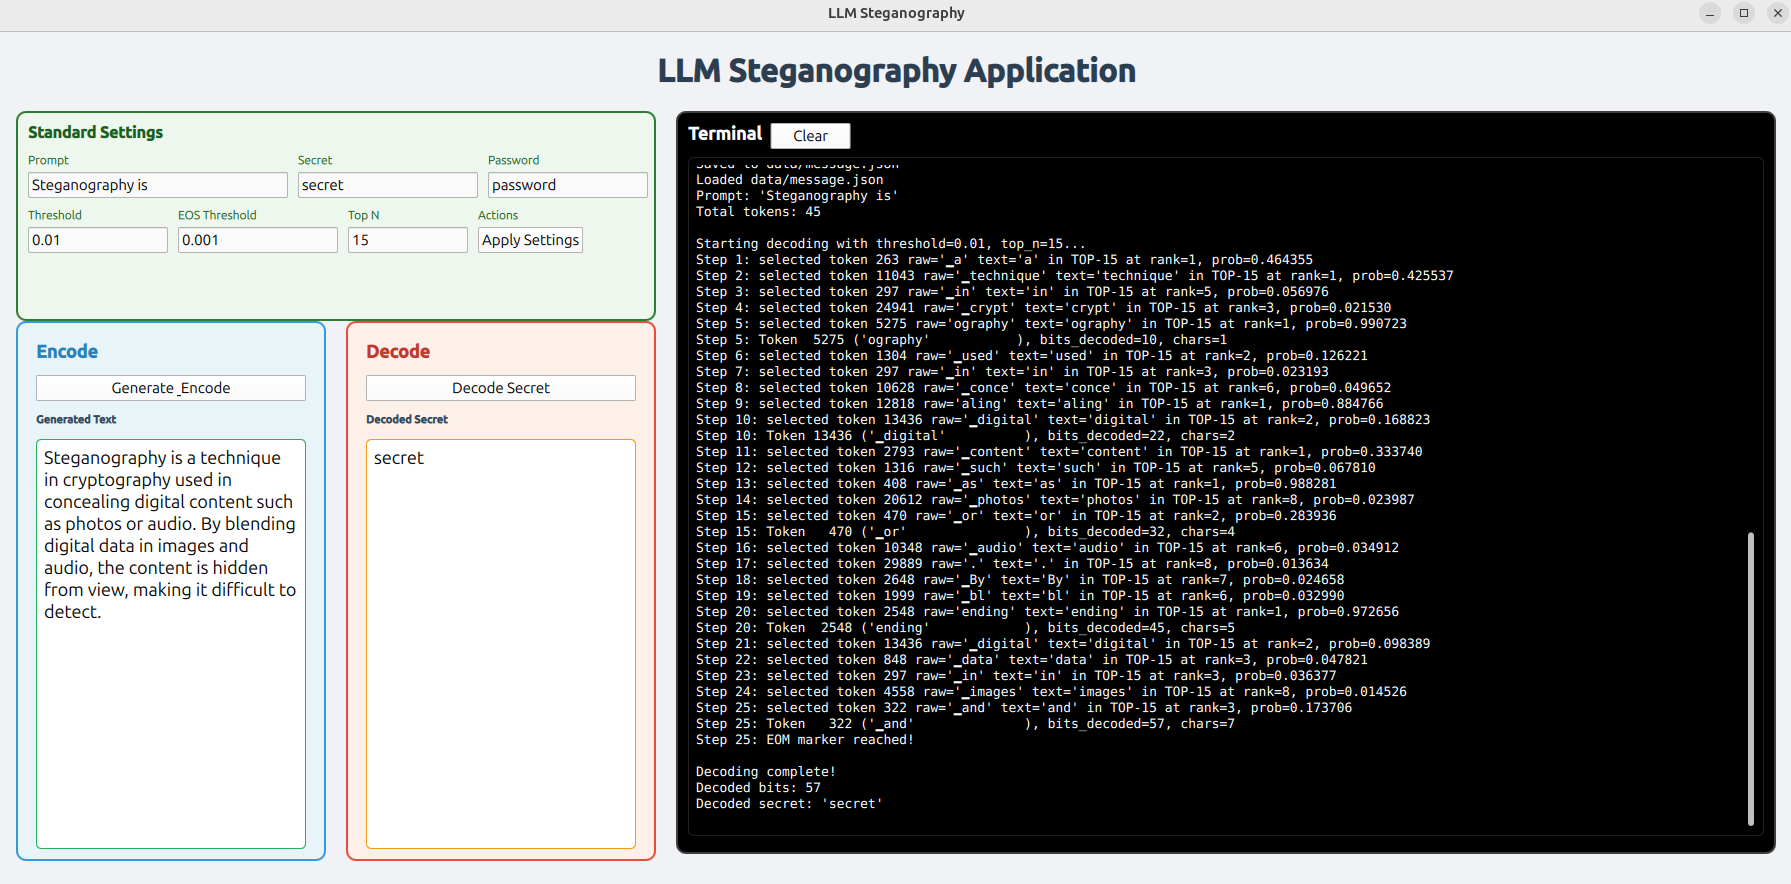
\includegraphics[width=0.98\linewidth]{app.png}
\caption{Widok aplikacji GUI z panelami Encode/Decode, ustawieniami oraz terminalem log\'ow}
\end{figure}

\subsection{Materiał demonstracyjny (wideo)}
Prezentacja działania aplikacji jest dostępna pod adresem:

\href{https://drive.google.com/file/d/19c5W6C8ZqfG-WvP81zaWk9ezISu9Fe-R/view?usp=sharing}{Film demonstracyjny projektu (Google Drive)}

\section{Uruchomienie}
Projekt można uruchomić lokalnie po zainstalowaniu zależności z pliku \texttt{requirements.txt}. Typowy scenariusz użycia wygląda następująco:
\begin{enumerate}
    \item uruchomienie aplikacji GUI poleceniem \texttt{python app.py},
    \item wpisanie promptu, sekretu, hasła i parametrów modelu,
    \item wygenerowanie tekstu steganograficznego,
    \item uruchomienie dekodowania i odczyt sekretu z pliku wyjściowego.
\end{enumerate}

W trybie tekstowym możliwe jest również bezpośrednie użycie modułów \texttt{encoder.py} i \texttt{decoder.py}, co ułatwia testowanie samego algorytmu bez GUI.

\section{Ograniczenia}
Rozwiązanie ma kilka istotnych ograniczeń:
\begin{itemize}
    \item nie zapewnia ochrony kryptograficznej -- bezpieczeństwo opiera się wyłącznie na ukryciu treści,
    \item dekodowanie wymaga dokładnie tych samych parametrów, co kodowanie,
    \item pojemność zależy od aktualnego rozkładu prawdopodobieństw tokenów,
    \item zmiana modelu lub parametrów próbkowania może uniemożliwić poprawne odtworzenie wiadomości,
\end{itemize}

\section{Wnioski}
Zrealizowany system pokazuje, że generatywny model językowy może posłużyć jako nośnik ukrytej wiadomości, jeśli wybór tokenów zostanie odpowiednio zdeterministycznie zakodowany. Najważniejszą cechą rozwiązania jest spójność między enkoderem i dekoderem: oba komponenty muszą wykonywać identyczne kroki, aby możliwe było odzyskanie sekretu.

Z perspektywy projektu osiągnięto zarówno część algorytmiczną, jak i użytkową. Algorytm demonstruje ideę steganografii w tekście generowanym przez LLM, a GUI upraszcza korzystanie z aplikacji i pozwala wygodnie sprawdzać działanie systemu.

\begin{thebibliography}{9}
\bibitem{readme} Dokumentacja projektu: \textit{README.md}.
\bibitem{pyqtreadme} Dokumentacja GUI: \textit{PYQT\_README.md}.
\bibitem{tinyllama} Model wykorzystywany w projekcie: TinyLlama-1.1B-Chat-v1.0.
\bibitem{demo} Film demonstracyjny projektu: \url{https://drive.google.com/file/d/19c5W6C8ZqfG-WvP81zaWk9ezISu9Fe-R/view?usp=sharing}.
\end{thebibliography}

\end{document}
